\documentclass[11pt]{article}
\usepackage{fontspec}
\usepackage{xeCJK}
\usepackage{xurl}
\usepackage[a4paper,margin=25mm]{geometry}
\usepackage{amsmath,amssymb,amsthm,mathtools}
\usepackage{xcolor}
\usepackage{booktabs,array,enumitem,fancyhdr,hyperref}
\hypersetup{colorlinks=true,linkcolor=blue!50!black,urlcolor=blue!50!black}
\setlength{\emergencystretch}{2em}
\setlength{\parskip}{0.3em}
\linespread{1.16}
\allowdisplaybreaks
\newtheorem{theorem}{定理}[section]
\newtheorem{proposition}[theorem]{命题}
\newtheorem{lemma}[theorem]{引理}
\theoremstyle{definition}
\newtheorem{definition}[theorem]{定义}
\theoremstyle{remark}
\newtheorem{remark}[theorem]{说明}
\newcommand{\dd}{\,\mathrm d}
\newcommand{\ii}{\mathrm i}
\newcommand{\Rea}{\operatorname{Re}}
\newcommand{\Ima}{\operatorname{Im}}
\newcommand{\Li}{\operatorname{Li}}
\newcommand{\supp}{\operatorname{supp}}
\pagestyle{fancy}
\fancyhf{}
\fancyhead[L]{\small 学习笔记}
\fancyhead[R]{\small 初稿}
\fancyfoot[C]{\thepage}
\setlength{\headheight}{15pt}
\author{}
\date{2026年10月22日初稿}
\makeatletter
\renewcommand{\maketitle}{%
  \thispagestyle{plain}%
  \begin{center}
    {\LARGE\bfseries \@title\par}
    \vspace{0.6em}
    {\small \@date\par}
  \end{center}
  \vspace{0.6em}}
\makeatother
\newcommand{\draftnotice}{\noindent{\small
本文为供逐篇审阅的学习笔记初稿，不是新增研究成果。
文中区分直接证明与引用结果；正文不依赖本文。
本轮已作公式、条件及排版初步核查，尚待作者逐句审定。}\par\medskip}

\usepackage{pgfplots}
\usepackage{float}
\pgfplotsset{compat=1.18}
\XeTeXlinebreaklocale "zh"
\renewcommand{\proofname}{证明}
\renewcommand{\figurename}{图}
\date{2026年10月26日初稿}
\title{经典零点自由区与余弦多项式类 $C_8$}
\begin{document}
\maketitle

\noindent{\small 本篇讨论 de la Vallée Poussin 型零点自由区（亦称零点禁区）中的常数，
说明它如何由一个非负余弦多项式决定，以及在 $8$ 次余弦多项式类 $C_8$ 中取最优时得到什么。
命题给出证明；所用的 $\zeta$ 的基本估计引用本书附录 F 与第 10 章；数值取自所引文献，并经独立复算。}\par\medskip

\section{问题}
本书附录 F 证明了经典零点自由区：存在常数 $R>0$，使
\begin{equation}
 \zeta(\sigma+it)\ne0\qquad\Bigl(\sigma>1-\frac1{R\log t},\ t\ \text{充分大}\Bigr).        \tag{1.1}
\end{equation}
$R$ 越小，自由区越宽。证明的关键是不等式 $3+4\cos\theta+\cos2\theta\ge0$。
本篇回答：这个三角多项式起什么作用；换成别的非负余弦多项式会怎样；在给定次数内能把 $R$ 压到多小。
文献中把满足一定条件的 $n$ 次余弦多项式全体记作 $C_n$；对 $n=8$，最优值已被确定（Tan 2025）。

\section{余弦多项式类 $C_n$ 与泛函 $v(f)$}
\begin{definition}
对整数 $n\ge2$，记 $C_n$ 为满足下列条件的余弦多项式
$f(\theta)=\sum_{k=0}^na_k\cos k\theta$ 的全体：
（A1）各 $a_k$ 为非负实数；（A2）$a_1>a_0>0$；（A3）对一切实数 $\theta$，$f(\theta)\ge0$。定义
\[
 v(f)=\frac{f(0)-a_0}{\bigl(\sqrt{a_1}-\sqrt{a_0}\bigr)^2},\qquad
 V_n=\inf_{f\in C_n}v(f).
\]
\end{definition}
由于 $C_n\subset C_{n+1}$（取 $a_{n+1}=0$），$V_n$ 关于 $n$ 不增。$v(f)$ 在 $f$ 乘以正数时不变。

\paragraph{经典例子} $3+4\cos\theta+\cos2\theta=2(1+\cos\theta)^2\ge0$，属于 $C_2$。此时 $a_0=3$，$a_1=4$，$f(0)=8$，
\[
 v=\frac{5}{(2-\sqrt3)^2}=69.641\ldots .
\]

\begin{figure}[H]
\centering
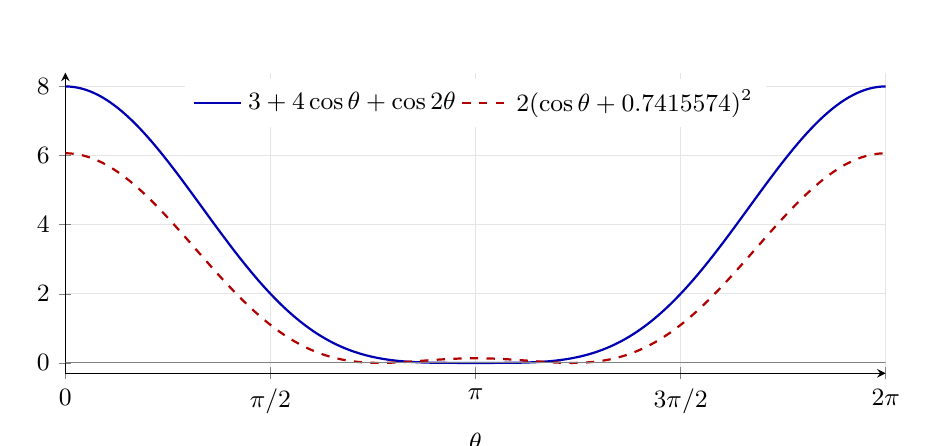
\begin{tikzpicture}
\begin{axis}[width=12cm,height=5.4cm,xmin=0,xmax=6.2832,ymin=-0.3,ymax=8.4,
 xtick={0,1.5708,3.1416,4.7124,6.2832},xticklabels={$0$,$\pi/2$,$\pi$,$3\pi/2$,$2\pi$},
 xlabel={$\theta$},grid=major,grid style={gray!20},axis lines=left,
 legend style={font=\small,draw=none,at={(0.5,0.98)},anchor=north},legend columns=2,
 tick label style={font=\small},label style={font=\small}]
\addplot[blue!70!black,thick,domain=0:6.2832,samples=200]{3+4*cos(deg(x))+cos(deg(2*x))};
\addlegendentry{$3+4\cos\theta+\cos2\theta$}
\addplot[red!70!black,thick,dashed,domain=0:6.2832,samples=200]{2*(cos(deg(x))+0.7415574)^2};
\addlegendentry{$2(\cos\theta+0.7415574)^2$}
\addplot[gray,thin,domain=0:6.2832]{0};
\end{axis}
\end{tikzpicture}
\caption{两个属于 $C_2$ 的非负余弦多项式。实线为经典选择，$v=69.64$；虚线为 $C_2$ 中的最优者（French），$v=V_2=53.139$。
两者都在 $\theta=\pi$ 附近接近或达到零；纵向缩放不影响 $v$。}
\label{fig:poly}
\end{figure}

\section{从 $f$ 到零点自由区}
\subsection{正性}
\begin{proposition}\label{prop:pos}
设 $f\in C_n$。则对 $\sigma>1$ 与实数 $t$，
\[
 \sum_{k=0}^na_k\Rea\Bigl(-\frac{\zeta'}{\zeta}(\sigma+ikt)\Bigr)\ge0 .
\]
\end{proposition}
\begin{proof}
$\sigma>1$ 时 $-\frac{\zeta'}{\zeta}(s)=\sum_m\Lambda(m)m^{-s}$ 绝对收敛，故
\[
 \Rea\Bigl(-\frac{\zeta'}{\zeta}(\sigma+ikt)\Bigr)=\sum_m\Lambda(m)m^{-\sigma}\cos(kt\log m).
\]
对 $k$ 加权求和并交换次序，得 $\sum_m\Lambda(m)m^{-\sigma}f(t\log m)\ge0$。
\end{proof}

\subsection{三项估计（引用）}
由 $\xi$ 的 Hadamard 乘积与 $\Gamma'/\Gamma$ 的渐近（本书第 10 章、附录 F），
对 $1<\sigma\le2$、$t\ge2$，
\begin{equation}
 -\Rea\frac{\zeta'}{\zeta}(\sigma+it)=\tfrac12\log t+O(1)-\sum_\rho\Rea\frac1{\sigma+it-\rho},     \tag{3.1}
\end{equation}
且其中每一项 $\Rea\frac1{\sigma+it-\rho}=\frac{\sigma-\beta}{|\sigma+it-\rho|^2}>0$。又
$-\frac{\zeta'}{\zeta}(\sigma)=\frac1{\sigma-1}+O(1)$（$1<\sigma\le2$）。
于是，丢掉 (3.1) 中全部零点项，得 $-\Rea\frac{\zeta'}{\zeta}(\sigma+ikt)\le\frac12\log t+O_n(1)$（$k\ge1$）；
若 $\rho_0=\beta_0+i\gamma_0$ 是零点、$t=\gamma_0$，只保留这一项，得
$-\Rea\frac{\zeta'}{\zeta}(\sigma+i\gamma_0)\le\frac12\log\gamma_0+O(1)-\frac1{\sigma-\beta_0}$。

\subsection{一个极小值}
\begin{lemma}\label{lem:min}
设 $0<a_0<a_1$，$\delta>0$。则
$\displaystyle\min_{x>0}\Bigl(\frac{a_0}x-\frac{a_1}{x+\delta}\Bigr)=-\frac{(\sqrt{a_1}-\sqrt{a_0})^2}{\delta}$，
在 $x^*=\delta\sqrt{a_0}/(\sqrt{a_1}-\sqrt{a_0})$ 处取到。
\end{lemma}
\begin{proof}
求导得 $a_0(x+\delta)^2=a_1x^2$，正根即 $x^*$。代入：
$a_0/x^*=\sqrt{a_0}(\sqrt{a_1}-\sqrt{a_0})/\delta$，$a_1/(x^*+\delta)=\sqrt{a_1}(\sqrt{a_1}-\sqrt{a_0})/\delta$，两者之差即所求。
函数在 $x\to0^+$ 时趋于 $+\infty$，$x\to\infty$ 时趋于 $0^-$，故该临界点是最小值点。
\end{proof}

\subsection{Landau 定理}
\begin{theorem}[Landau]\label{thm:landau}
设 $f\in C_n$，$\varepsilon>0$。则存在 $T_0$，使每个满足 $\gamma\ge T_0$ 的非平凡零点 $\beta+i\gamma$ 都有
\[
 1-\beta\ge\Bigl(\frac{2}{v(f)}-\varepsilon\Bigr)\frac1{\log\gamma}.
\]
换言之，对充分大的 $t$，(1.1) 对任意 $R>v(f)/2$ 成立。
\end{theorem}
\begin{proof}
取 $t=\gamma$，$\sigma=1+x/\log\gamma$（$x>0$ 待定），记 $\delta=(1-\beta)\log\gamma$。
在命题~\ref{prop:pos} 中，$k=0$ 项用 $\frac1{\sigma-1}+O(1)$，$k=1$ 项只保留零点 $\rho$，$k\ge2$ 项丢掉全部零点。
由 $\sum_{k\ge1}a_k=f(0)-a_0$，
\[
 0\le\frac{a_0}{\sigma-1}-\frac{a_1}{\sigma-\beta}+\frac{f(0)-a_0}2\log\gamma+O_f(1).
\]
除以 $\log\gamma$，并注意 $\sigma-1=x/\log\gamma$，$\sigma-\beta=(x+\delta)/\log\gamma$：
\[
 0\le\frac{a_0}{x}-\frac{a_1}{x+\delta}+\frac{f(0)-a_0}2+O_f\Bigl(\frac1{\log\gamma}\Bigr).
\]
取 $x=x^*$（引理~\ref{lem:min}；$\gamma$ 足够大时 $1<\sigma\le2$），得
\[
 \frac{(\sqrt{a_1}-\sqrt{a_0})^2}{\delta}\le\frac{f(0)-a_0}2+O_f\Bigl(\frac1{\log\gamma}\Bigr),
 \quad\text{即}\quad
 \delta\ge\frac{2}{v(f)}-O_f\Bigl(\frac1{\log\gamma}\Bigr).
\]
\end{proof}

\begin{figure}[H]
\centering
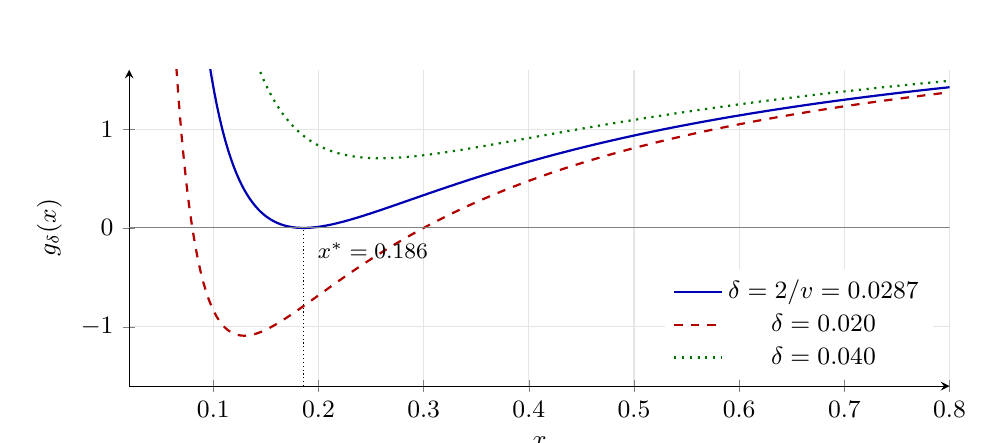
\begin{tikzpicture}
\begin{axis}[width=12cm,height=5.6cm,xmin=0.02,xmax=0.8,ymin=-1.6,ymax=1.6,
 xlabel={$x$},ylabel={$g_\delta(x)$},grid=major,grid style={gray!20},axis lines=left,
 legend style={font=\small,draw=none,at={(0.98,0.02)},anchor=south east},
 tick label style={font=\small},label style={font=\small}]
\addplot[blue!70!black,thick,domain=0.02:0.8,samples=300]{3/x-4/(x+0.0287187)+2.5};
\addlegendentry{$\delta=2/v=0.0287$}
\addplot[red!70!black,thick,dashed,domain=0.02:0.8,samples=300]{3/x-4/(x+0.02)+2.5};
\addlegendentry{$\delta=0.020$}
\addplot[green!45!black,thick,dotted,domain=0.02:0.8,samples=300]{3/x-4/(x+0.04)+2.5};
\addlegendentry{$\delta=0.040$}
\addplot[gray,thin,domain=0.02:0.8]{0};
\draw[densely dotted] (axis cs:0.18564,-1.6)--(axis cs:0.18564,0);
\node[font=\footnotesize,anchor=north west] at (axis cs:0.19,-0.05) {$x^*=0.186$};
\end{axis}
\end{tikzpicture}
\caption{对 $f=3+4\cos\theta+\cos2\theta$，$g_\delta(x)=\frac3x-\frac4{x+\delta}+\frac52$（定理~\ref{thm:landau} 证明中略去 $O(1/\log\gamma)$ 后的主部）。
若零点的规范距离 $\delta=(1-\beta)\log\gamma$ 小于 $2/v=0.0287$，则 $g_\delta$ 取到负值（虚线），与正性矛盾；
$\delta=2/v$ 时最小值恰为零（实线）。这正是常数 $R=v/2$ 的来源。}
\label{fig:g}
\end{figure}

\section{$C_2$ 到 $C_8$ 的最优值}
按定理~\ref{thm:landau}，经典多项式给出 $R=v/2=34.82$。在各 $C_n$ 中最优化：
\begin{center}
\small
\begin{tabular}{cccl}
\toprule
$n$ & $V_n$ & $R=V_n/2$ & 出处\\
\midrule
$2$ & $53.1390720$ & $26.57$ & French；最优者为 $(\cos\theta+0.7415574)^2$\\
$3$ & $36.9199911$ & $18.46$ & Arestov\\
$4,5,6$ & $34.8992259$ & $17.45$ & Arestov\\
$7$ & $34.6494874$ & $17.32$ & Tan 2025\\
$8$ & $34.5399155$ & $17.27$ & Tan 2025\\
\bottomrule
\end{tabular}
\end{center}
（表中数值取自 Tan 2025；$C_2$ 一行的 $v$ 值经本文复算为 $53.1390720$。）
从 $C_2$ 到 $C_3$ 改进显著，此后改进很慢：$V_4=V_5=V_6$，$V_8$ 只比 $V_4$ 小约 $1\%$。
这说明在 Landau 的框架内，单纯提高余弦多项式的次数，所能得到的 $R$ 大约停在 $17$ 附近。

\section{$C_8$ 的位置：方法的极限与现代纪录}
文献中 $R$ 的历史值（Tan 2025 表 1 汇总）：
\begin{center}
\small
\begin{tabular}{lll}
\toprule
年份 & 作者 & $R$\\
\midrule
1899 & de la Vallée Poussin & $30.47$\\
1962 & Rosser--Schoenfeld & $17.52$\\
1970 & Stechkin & $9.65$\\
2005 & Kadiri & $5.69$\\
2024 & Mossinghoff--Trudgian--Yang & $5.558691$（对一切 $t\ge2$ 显式成立）\\
\bottomrule
\end{tabular}
\end{center}
Stechkin 以后的改进都超出了定理~\ref{thm:landau} 的框架：
\begin{itemize}
 \item Stechkin 利用零点关于临界线的对称性（$\rho$ 与 $1-\bar\rho$ 同为零点），
 不再把 (3.1) 中其余零点的贡献全部丢掉，从而把常数从 $17.52$ 降到 $9.65$；
 \item Kadiri 等人用光滑权重代替直接取 $-\zeta'/\zeta$ 的值，并结合有限高度上已验证的 RH，
 进一步把 $R$ 压到 $6$ 以下。
\end{itemize}
因此 $V_8/2=17.27$ 不是零点自由区常数的最好值，而是“只改进余弦多项式”这一方向的精确界限；
它的意义在于说明：要越过这个界限，必须改用更多的零点信息或光滑化等新的工具。

\paragraph{一个下界} 由附录 F 中关于经典零点自由区常数的注，第一个零点 $\tfrac12+14.1347i$ 本身就要求 $R\ge2/\log\gamma_1=0.7551$；
若 RH 成立，最优常数恰为此值。现有纪录 $5.56$ 与这个下界之间，仍相差约 $7$ 倍。

\begin{figure}[H]
\centering
\begin{tikzpicture}
\begin{loglogaxis}[width=12.5cm,height=6.4cm,xmin=14,xmax=1e12,ymin=2e-4,ymax=0.9,
 xlabel={$t$},ylabel={自由区宽度 $1-\sigma=1/(R\log t)$},grid=major,grid style={gray!20},axis lines=left,
 legend style={font=\small,draw=none,at={(0.5,-0.22)},anchor=north,/tikz/every even column/.append style={column sep=1.2em}},legend columns=2,
 tick label style={font=\small},label style={font=\small}]
\addplot[green!45!black,thick,dotted,domain=14.1347:1e12,samples=200]{1/(0.755106*ln(x))};
\addlegendentry{$R=0.755$（第一零点给出的下界）}
\addplot[red!70!black,thick,domain=14:1e12,samples=200]{1/(5.558691*ln(x))};
\addlegendentry{$R=5.56$（2024 年纪录）}
\addplot[blue!70!black,thick,dashed,domain=14:1e12,samples=200]{1/(17.26996*ln(x))};
\addlegendentry{$R=17.27$（$C_8$ 最优）}
\addplot[black,thick,domain=14:1e12,samples=200]{1/(34.8205*ln(x))};
\addlegendentry{$R=34.82$（$3+4\cos\theta+\cos2\theta$）}
\addplot[gray,thin,domain=14:1e12]{0.5};
\end{loglogaxis}
\end{tikzpicture}
\caption{零点自由区的宽度 $1/(R\log t)$，即自由区边界到直线 $\Rea s=1$ 的距离（双对数刻度）。
宽度随 $t$ 增大而趋于零：经典零点自由区只刻画 $\Rea s=1$ 附近的情形，与临界线（灰色横线，宽度 $\tfrac12$）相距甚远。
点线在 $t=\gamma_1$ 处恰等于 $\tfrac12$。各曲线互相平行，相差的只是常数倍 $R$。}
\label{fig:regions}
\end{figure}

\section{结论}
\begin{enumerate}
 \item 经典零点自由区的常数由一个非负余弦多项式 $f$ 决定：$R=v(f)/2$（Landau）。
 其来源是 $\sum a_k\Rea(-\zeta'/\zeta)$ 的正性与一个一元极小值问题。
 \item 在 $8$ 次余弦多项式类 $C_8$ 中取最优，得到 $R=V_8/2\approx17.27$；
 提高次数的收益在 $n\ge4$ 后已很小。
 \item 现代纪录 $R\approx5.56$ 来自 Landau 框架之外的工具；而 RH 所对应的最优常数是 $0.755$。
 更新的预印本（2026 年 3 月）声称对 $t\ge3$ 可取 $R=4.896$，尚待核验。
 \item 无论 $R$ 多小，这类自由区都只说明零点离开直线 $\Rea s=1$ 的程度，不涉及临界线本身。
\end{enumerate}

\section*{参考}
\begin{itemize}
 \item H.\ S.\ Tan, Optimal cosine polynomials for Riemann zeta zero-free region, 2025. \url{https://arxiv.org/abs/2411.01385}
 \item M.\ J.\ Mossinghoff, T.\ S.\ Trudgian, A.\ Yang, Explicit zero-free regions for the Riemann zeta-function, \emph{Res.\ Number Theory} 10 (2024), Art.~11.
 \item Zero-free regions inspired by work of Heath-Brown, 2026（预印本）. \url{https://arxiv.org/abs/2603.21490}
 \item H.\ Kadiri, Une région explicite sans zéros pour la fonction $\zeta$ de Riemann, \emph{Acta Arith.} 117 (2005)。
 \item E.\ C.\ Titchmarsh, \emph{The Theory of the Riemann Zeta-Function}, 2nd ed., 1986, Ch.~III。
 \item 本书第 10 章（Hadamard 乘积）、附录 F（零点自由区及注“经典零点自由区常数”）。
\end{itemize}
\end{document}
